\documentclass{article}
\usepackage{graphicx}
\usepackage[margin=1.5cm]{geometry}
\usepackage{amsmath}

\begin{document}

\title{Wednesday Reading Assessment: Unit 3, Magnetic Forces and Fields}
\author{Prof. Jordan C. Hanson}

\maketitle

\section{Memory Bank}

\begin{itemize}
\item $\vec{F} = I\vec{L} \times \vec{B}$ ... Force on a current-carrying wire.
\item $\vec{F} = q\vec{v} \times \vec{B}$ ... Force on a charged particle in a B-field.
\item $U = q\Delta V$ ... Potential energy gained by a charge proceeding through a potential.
\item $KE = \frac{1}{2}mv^2$ ... Kinetic energy.
\end{itemize}

\begin{figure}[ht]
\centering
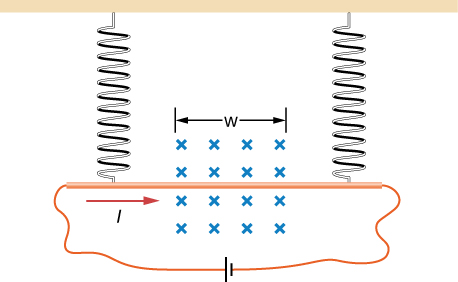
\includegraphics[width=0.3\textwidth]{currentBfieldSpring.jpeg} \hspace{0.2cm}
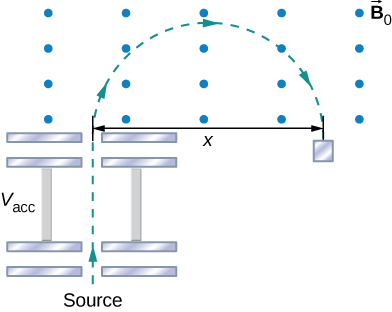
\includegraphics[width=0.3\textwidth]{massSpec.jpeg}
\caption{\label{fig:fields} (Left) A current I causes a force on the wire such that the spring tension is eased. (Right) A schematic of a mass spectrometer.}
\end{figure}

\section{Magnetic Forces on a Wire}

\begin{enumerate}
\item Consider Fig. \ref{fig:fields} (left). A metal rod of mass $m$ and length $L$ is hung from the ceiling using two springs of spring constant $k$. A uniform magnetic field of magnitude $B$ pointing perpendicular to the rod and spring exists in a region of space covering a length $w$ of the copper rod. The ends of the rod are then connected by flexible copper wire across the terminals of a battery. Determine the change in the length of the springs when a current $I$ runs through the copper rod, in terms of the other given variables. \textit{Check units, and take limits...do the results make sense?} \\ \vspace{2.5cm}
\item A schematic for a device called a \textit{mass spectrometer} that measures the mass of ions is shown in Fig. \ref{fig:fields} (right). An ion of mass $m$ and charge $q$ is at rest and accelerated by a potential difference $V_{\rm acc}$ and allowed to enter a region of constant magnetic field $B_0$.  In the uniform magnetic field region, the ion moves in a semicircular path striking a photographic plate at a distance $x$ from the entry point.  Derive a formula for $x$ in terms of the other given variables.
\end{enumerate}

\end{document}
